% Fontawesome: Ready Icons to Use in LaTeX!
% TikZ example
% Latexdraw.com
% 21/01/2021, 02:31

\documentclass[border=0.1cm]{standalone}
\usepackage[dvipsnames]{xcolor}
\usepackage{tikz}
\usepackage{fontawesome5}



\begin{document}

\begin{tikzpicture}

\node[scale=4,Goldenrod] at (0,0){\faIcon{trophy}};
\node[scale=4,SpringGreen] at (3,0){\faIcon{university}};
\node[scale=4,OliveGreen] at (6,0){\faIcon{twitter}};
\node[scale=4,Green] at (9,0){\faIcon{researchgate}};
\node[scale=4,Red] at (12,0){\faIcon{address-card}};
\node[scale=4,BlueGreen] at (15,0){\faIcon{book}};
\node[scale=4,Cyan] at (18,0){\faIcon{at}};

\begin{scope}[yshift=-3cm]
\node[scale=4,RoyalBlue] at (0,0){\faIcon{code}};
\node[scale=4,Violet] at (3,0){\faIcon{phone-square-alt}};
\node[scale=4,Orchid] at (6,0){\faIcon{file-alt}};
\node[scale=4,Fuchsia] at (9,0){\faIcon{orcid}};
\node[scale=4,RedViolet] at (12,0){\faIcon{mobile-alt}};
\node[scale=4,LimeGreen] at (15,0){\faIcon{calendar-alt}};
\node[scale=4,CarnationPink] at (18,0){\faIcon{map-marker-alt}};
\end{scope}

\begin{scope}[yshift=-6cm]
\node[scale=4,Blue] at (0,0){\faIcon{linkedin}};
\node[scale=4,Rhodamine] at (3,0){\faIcon{link}};
\node[scale=4,Green] at (6,0){\faIcon{google}};
\node[scale=4,OrangeRed] at (9,0){\faIcon{google-plus}};
\node[scale=4,RedOrange] at (12,0){\faIcon{github}};
\node[scale=4,Salmon] at (15,0){\faIcon{envelope}};
\node[scale=4,Dandelion] at (18,0){\faIcon{youtube}};
\end{scope}

\end{tikzpicture}
\end{document}
